\documentclass[tikz]{standalone}
\usepackage{tikz}
\usepackage{alphalph}
\usetikzlibrary{positioning, graphs}
\usetikzlibrary{graphs.standard}
\begin{document}
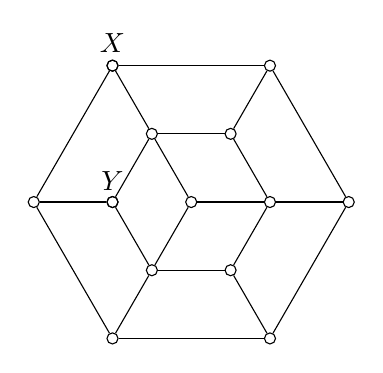
\begin{tikzpicture}
\begin{scope}
		[every node/.style={draw,circle,inner sep = 0em, minimum size = 0.4em},
		 edgelabel/.style = {fill = white, inner sep = 0.1em, font=\small}]
		
		\graph[clockwise, radius = 2cm, phase = 0, empty nodes]{subgraph C_n[n = 6, name = A]};
		\graph[clockwise, radius = 1cm, phase = 0, empty nodes]{subgraph C_n[n = 6, name = B]};
		
		\node[label={$X$}] (a) at (A 5) {};
		\node[label={$Y$}] (b) at (B 4) {};
		
%		\node[fill=blue] (d) at (B 1) {};
%		\node[fill=blue] (e) at (B 3) {};
%		\node[fill=blue] (f) at (B 5) {};
%		\node[fill=blue] (g) at (A 2) {};
%		\node[fill=blue] (h) at (A 4) {};
%		\node[fill=blue] (i) at (A 6) {};
		
		\draw (0,0) node (c) {};
		
		\foreach \i in {1, 2, 3, 4, 5, 6}{
			\draw[-] (A \i) to (B \i);
		}
		
		\draw[-] (c) to (B 1);
		\draw[-] (c) to (B 3);
		\draw[-] (c) to (B 5);
		
%		\draw[red, thick] (A 5) to (B 4);
%		\draw[red, thick] (B 4) to (A 4);
%		\draw[red, thick] (A 4) to (A 3);
%		\draw[red, thick] (A 3) to (B 3);
%		\draw[red, thick] (B 3) to (c);
%		\draw[red, thick] (c) to (B 5);
%		\draw[red, thick] (B 5) to (B 6);
%		\draw[red, thick] (B 6) to (B 1);
%		\draw[red, thick] (B 1) to (B 2);
%		\draw[red, thick] (B 2) to (A 2);
%		\draw[red, thick] (A 2) to (A 1);
%		\draw[red, thick] (A 1) to (A 6);
%		\draw[red, thick] (A 6) to (A 5);
		
\end{scope}
\end{tikzpicture}
\end{document}